
The stated long term plan for nuclear deployment in France targets a technology 
transition to \glspl{SFR} \cite{cne2_reports_2015}. However, the current inventory of French \gls{UNF} 
is insufficient to fuel that transition without building new \glspl{LWR} \cite{carre_overview_2009}.

If instead, France accepted 
\gls{UNF} from other \gls{EU} nations and used it to produce \gls{MOX} for new \glspl{SFR},
the \gls{MOX} created will fuel a French transition to an \gls{SFR} fleet
and allow France to avoid building additional \glspl{LWR}.

To simulate this cooperative scenario, I simulated the entire \gls{EU} region
and all its nuclear reactor operating history and \gls{UNF} accumulation up to the
nearest foreseeable future. Then, France takes as much \gls{UNF} it needs
to transition into a fully \gls{SFR} fleet without building additional \glspl{LWR}.

This chapter includes the results from a French \gls{NFC} transition
scenario from a \gls{LWR} fleet to a fully \gls{SFR} fleet by
taking other \gls{EU} nations' \gls{UNF}.


\section{\gls{EU} Deployment Schedule}

The historic \gls{EU} deployment schedule and operation history 
are generated using the \texttt{write\_input.py}
module (described in section \ref{sec:writeinput}).

Projections of future reactor deployment in this simulation are based on
assessment of analyses from references, for instance \gls{PRIS}, for reactors planned
for construction \cite{iaea_nuclear_2017}, the World Nuclear Association
\cite{world_nuclear_association_nuclear_2017}, and literature concerning the future of
nuclear power in a global \cite{joskow_future_2012} and European context
\cite{hatch_politics_2015}.  Existing projections extend to 2050.

\Cref{tab:eu_deployment} lists the reactors that are currently  planned or
under construction in the \gls{EU}. In the simulation, all  planned constructions are completed 
without delay or failure and reach a lifetime of 60 years.  

\pagebreak
\begin{table}[h]
    \centering
    \caption {Power reactors under construction and planned. Replicated from \cite{world_nuclear_association_nuclear_2017}.}
    \label{tab:eu_deployment}
    \begin{tabular}{ccccr}
        \hline
        \textbf{Exp. Operational }&\textbf{Country} &\textbf{Reactor} & \textbf{Type} & \textbf{Gross \gls{MWe}}\\
        \hline
        2018 & Slovakia  & Mochovce 3 & PWR & 440\\
        2018 & Slovakia & Mochovce 4 & PWR & 440 \\
        2018 & France & Flamanville 3 & PWR & 1600 \\
        2018 & Finland & Olkilouto 3 & PWR & 1720 \\
        2019 & Romania & Cernavoda 3 & PHWR & 720 \\
        2020 & Romania & Cernavoda 4 & PHWR & 720 \\
        2024 & Finland & Hanhikivi & VVER1200 & 1200 \\
        2024 & Hungary & Paks 5 & VVER1200 & 1200 \\
        2025 & Hungary & Paks 6 & VVER1200 & 1200 \\
        2025 & Bulgaria & Kozloduy 7 & \footnotemark AP1000 & 950 \\
        2026 & UK & Hinkley Point C1 & EPR & 1670 \\
        2027 & UK & Hinkley Point C2 & EPR & 1670 \\
        2029 & Poland & Choczewo & N/A & 3000 \\
        2035 & Poland & N/A & N/A & 3000 \\
        2035 & Czech Rep & Dukovany 5 & N/A & 1200 \\
        2035 & Czech Rep & Temelin 3 & AP1000 & 1200 \\
        2040 & Czech Rep & Temelin 4 & AP1000 & 1200 \\
        \hline
    \end{tabular}
\end{table}

    \footnotetext{The fate of many planned reactors is uncertain. The proposed reactor types
              are also unclear. The ones marked `N/A' for type are assumed to the \glspl{PWR}
              in the simulation.}
\FloatBarrier

For each \gls{EU} nation, we categorize the growth trajectory from
``Aggressive Growth'' to ``Aggressive Shutdown''. ``Aggressive growth'' is
characterized by a rigorous expansion of nuclear power, while
``Aggressive Shutdown'' is characterized as a transition to rapidly
de-nuclearize the nation's electric grid. We categorize each nation's growth 
trajectory into five degrees depending on G, the growth trajectory metric:

 \[
 G = \left\{\begin{array}{ll}
 \text{Aggressive Growth}, & \text{for } G \geq 2\\
 \text{Modest Growth}, & \text{for } 1.2 \leq G < 2\\
 \text{Maintanence}, & \text{for } 0.8 \leq G < 1.2 \\
 \text{Modest Reduction}, & \text{for } 0.5 \leq G< 0.8\\
 \text{Aggressive Reduction}, & \text{for } G \leq 0.5
 \end{array}\right\} = \frac{C_{2040}}{C_{2017}}\\\\
 \]
 \[
  G = \text{Growth Trajectory  } [-] 
 \]
 \[
 C_{i} = \text{Nuclear Capacity in Year i  } [\gls{MWe}].
 \]

The growth trajectory and specific plan of each nation in the \gls{EU} 
is listed in Table \ref{tab:eu_growth}.  

\begin{table}[h]
    \centering
    \caption{Projected nuclear power strategies of \gls{EU} nations \cite{world_nuclear_association_nuclear_2017}}
        \begin{tabular}{lll}
            \hline 
                    \textbf{Nation} & \textbf{Growth Trajectory} & \textbf{Specific Plan }\\
                    \hline
                    UK & Aggressive Growth & {\small  13 units (17,900 \gls{MWe}) by 2030.}\\
                    Poland & Aggressive Growth &  {\small Additional 6,000 \gls{MWe} by 2035.}\\
                    Hungary & Aggressive Growth &  {\small Additional 2,400 \gls{MWe} by 2025.} \\ 
                    Finland & Modest Growth &  {\small Additional 2,920 \gls{MWe} by 2024.}\\
                    Slovakia & Modest Growth & {\small Additional 942 \gls{MWe} by 2025.}\\
                    Bulgaria & Modest Growth &  {\small Additional 1,000 \gls{MWe} by 2035.} \\
                    Romania & Modest Growth &  {\small Additional 1,440 \gls{MWe} by 2020.} \\
                    Czech Rep. & Modest Growth & {\small  Additional 2,400 \gls{MWe} by 2035.}\\
                    France & Modest Reduction & {\small No expansion or early shutdown.}\\
                    Slovenia & Modest Reduction & {\small No expansion or early shutdown.}\\
                    Netherlands & Modest Reduction & {\small No expansion or early shutdown.}\\
                    Lithuania & Modest Reduction & {\small No expansion or early shutdown.}\\
                    Spain & Modest Reduction &  {\small No expansion or early shutdown.} \\
                    Italy & Modest Reduction & {\small No expansion or early shutdown. }\\
                    Belgium & Aggressive Reduction & All shut down 2025.\\
                    Sweden & Aggressive Reduction & All shut down 2050.\\
                    Germany & Aggressive Reduction & All shut down by 2022.\\
                    \hline
                    
        \end{tabular}
  \label{tab:eu_growth}
\end{table}
\FloatBarrier


Using this categorization to drive facility deployment, Cyclus captures 
regional differences in reactor power capacity and \gls{UNF} production as a 
function of time. Accordingly, \cref{fig:eu_pow} shows the resulting simulated 
installed capacity in \gls{EU} nations.  Sudden capacity reductions seen in the 
2040s result from end-of-license reactor retirements and nuclear phaseout plans 
in nations such as Germany and Belgium.  

\begin{figure}[htbp!]
    \begin{center}
        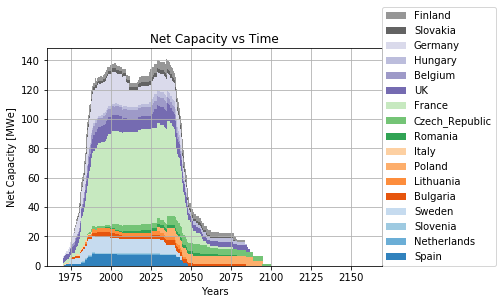
\includegraphics[scale=0.7]{./images/eu_future/power_plot.png}
    \end{center}
    \caption{Installed nuclear capacity in the EU is distinguished by \texttt{Region}s in \Cyclus.}
    \label{fig:eu_pow}
\end{figure}


\section{French \gls{SFR} Deployment Schedule}

\Cref{fig:sfr_num}
shows
the French transition to \glspl{SFR} modeled in this simulation.
Historically aggressive growth of nuclear in the 1980s leads to a substantial 
shutdown of nuclear in the 2040s, which, in the simulation, are replaced by new 
\glspl{SFR}. The net capacity is kept constant at 66 GWe.

\begin{figure}[htbp!]
        \begin{center}
                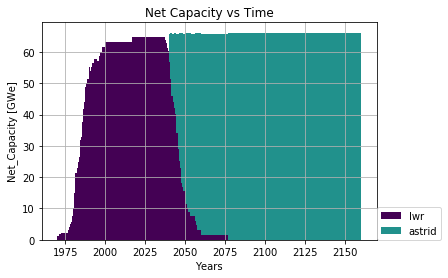
\includegraphics[scale=0.7]{./images/french-transition/power_plot.png}
        \end{center}
        \caption{The potential French transition from \glspl{LWR} to 
                \glspl{SFR} when assisted by \gls{UNF} from other \gls{EU} 
        nations.}
        \label{fig:sfr_num}
\end{figure}

\Cref{fig:french_dep} shows the deployment strategy required to support the transition in 
\cref{fig:sfr_num}. France must build four reactors per year, on average, to 
make up for the end-of-license decommissioning of power plants built in the 1980s and 1990s.  The second period of aggressive building occurs when the first generation of \glspl{SFR} decommission after 80 years. Starting in 2040, France deploys 600-\gls{MWe} \glspl{SFR} to make up for 
decommissioned French \gls{LWR} capacity. This results in an installed 
\gls{SFR} 
capacity of 66,000 \gls{MWe} by 2078 when the final \gls{LWR} is 
decommissioned. 



\begin{figure}[htbp!]
    \begin{center}
        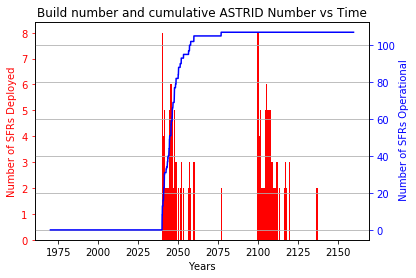
\includegraphics[scale=0.7]{./images/french-transition/sfr_deploy.png}
    \end{center}
    \caption{The simulated deployment of \glspl{SFR} in France is characterized by a period of
    aggressive building.}
    \label{fig:french_dep}
\end{figure}


Finally, \Cref{fig:tot_dep} shows the total deployment scheme we simulated.  
The French transition to \glspl{SFR} couples with the historical and projected 
operation of \gls{EU} reactors.  The steep transition from 2040 to 2060 
reflects the scheduled decommissioning of reactors built in the 1975-2000 era 
of aggressive nuclear growth in France.

\begin{figure}[htbp!]
    \begin{center}
        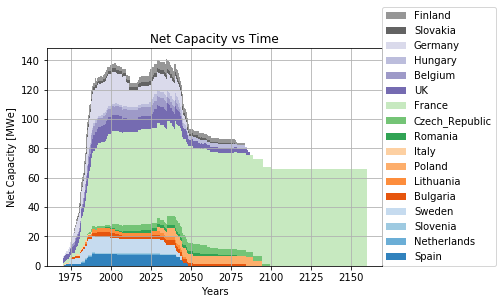
\includegraphics[scale=0.7]{./images/eu_future/onesim.png}
    \end{center}
    \caption{The total simulated deployment scheme relies on \gls{UNF} 
    collaboration among nations.} 
    \label{fig:tot_dep}
\end{figure}

These figures reflect that, for the given assumptions, bursts of construction
are necessary to maintain capacity.  In reality, a construction rate of five 
reactors every year is ambitious, but might have the advantage of
larger scale production of components and more modular assembly and construction if major components can mostly be built off site.

Alternatively, the 
deployment of new \glspl{SFR} can be spread out by staggering scheduled 
decommissioning of \glspl{LWR} through lifetime extensions. For example,
I increased the original lifetime of French \glspl{LWR} (60 years) randomly 
by sampling from a uniform distribution of lifetime extension
magnitudes between 0 and 25 years. 
This results in a more gradual transition and \gls{ASTRID} construction
burden, as shown in figure \ref{fig:sfr_num_norm} and \ref{fig:sfr_dep_norm}.
The effect of \gls{LWR} lifetime extension is discussed in Section \ref{sec:life}.

\begin{figure}[htbp!]
	\begin{center}
		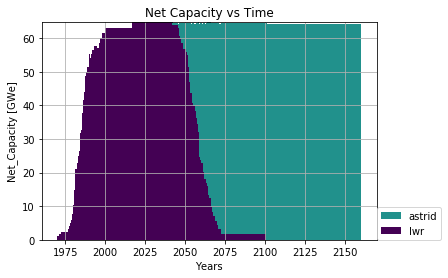
\includegraphics[scale=0.7]{./images/french-transition/unif_0_25.png}
	\end{center}
	\caption{The transition to \glspl{ASTRID}
		becomes more gradual if the
		French \glspl{LWR} lifetime extensions are sampled from a 
		uniform distribution $\in [0, 25]$ years.}
	\label{fig:sfr_num_norm}
\end{figure}

\begin{figure}[htbp!]
	\begin{center}
		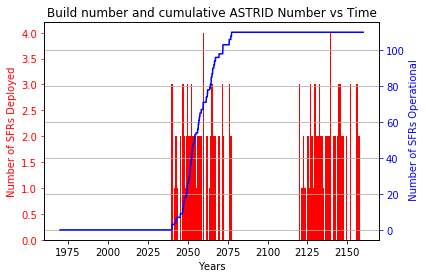
\includegraphics[scale=0.7]{./images/french-transition/unif_0_25_dep.png}
	\end{center}
	\caption{The acute construction burden lessens if the
		French \glspl{LWR} lifetime extensions are sampled from a 
		uniform distribution $\in [0, 25]$ years.}
	\label{fig:sfr_dep_norm}
\end{figure}

\FloatBarrier

This analysis establishes a multi-national material flow and demonstrates that, if such an aggressive deployment scheme took place, the \glspl{SFR} would have enough fuel.

\section{Material Flow}

The fuel cycle is represented by a series of facility agents whose material 
flow is illustrated in figure \ref{diag:fc}, along with
the \Cyclus archetypes that were used to model each facility.
In this diagram, \gls{MOX} Reactors include both French \glspl{PWR} and 
\glspl{SFR}.

% Define block styles
\tikzstyle{decision} = [diamond, draw, fill=blue!20, 
text width=4.5em, text badly centered, node distance=3cm, inner sep=0pt]
\tikzstyle{block} = [rectangle, draw, fill=blue!20, 
text width=5em, text centered, rounded corners, minimum height=4em]
\tikzstyle{line} = [draw, -latex']
\tikzstyle{cloud} = [draw, ellipse,fill=red!20, node distance=3cm,
minimum height=2em]


\begin{figure}
	\centering
	\scalebox{0.6}{
		\begin{tikzpicture}[align=center, node distance = 3cm and 3cm, auto]
		% Place nodes
		\node [block] (sr) {Mine (\texttt{SOURCE})};
		\node [cloud, below of=sr] (nu) {Nat U};
		\node [block, below of=nu] (enr) {Enrichment ({\footnotesize \texttt{ENRICHMENT}})};
		\node [cloud, below of=enr] (uox) {\acrshort{UOX}};
		\node [block, below of=uox] (lwr) {\gls{LWR} (\texttt{REACTOR})};
		\node [cloud, right of=lwr] (snf) {\gls{UNF}};
		\node [block, right of=snf] (pool) {Pool (\texttt{Storage})};
		\node [cloud, left of=lwr] (tl2) {Dep U};
		\node [cloud, right of=enr] (tl) {Dep U};
		\node [block, right of=tl] (sk) {Repository (\texttt{SINK})};
		\node [cloud, below of=sk] (cunf) {Cooled \gls{UNF}};
		\node [cloud, below of=pool] (cunf2) {Cooled \gls{UNF}};
		\node [block, below of=snf] (rep) {{\small Reprocessing ({\footnotesize \texttt{SEPARATIONS}})}};
		\node [cloud, below of=rep] (u) {Sep. U} ;
		\node [cloud, left of=rep] (pu) {Sep. Pu};
		\node [block, left of=pu] (mix) {Fabrication (\texttt{MIXER})};
		\node [cloud, below of=mix] (mox) {\gls{MOX}};
		\node [block, below of=mox] (mxr) {\gls{MOX} Reactors 
			(\texttt{REACTOR})};
		\node [cloud, right of= mxr] (snmox) {Spent \gls{MOX}};
		
		\draw[->, thick] (sr) -- (nu);
		\draw[->, thick] (nu) -- (enr);
		\draw[->, thick] (enr) -- (tl);
		\draw[->, thick] (enr) -- (tl2);
		\draw[->, thick] (tl) -- (sk);
		\draw[->, thick] (tl2) -- (mix);
		\draw[->, thick] (enr) -- (uox);
		\draw[->, thick] (uox) -- (lwr);
		\draw[->, thick] (lwr) -- (snf);
		
		\draw[->, thick] (lwr) -- (snf);
		\draw[->, thick] (snf) -- (pool);
		\draw[->, thick] (pool) -- (cunf);
		\draw[->, thick] (pool) -- (cunf2);
		\draw[->, thick] (cunf) -- (sk);
		\draw[->, thick] (cunf2) -- (rep);
		
		\draw[->, thick] (rep) -- (u);
		\draw[->, thick] (rep) -- (pu);
		\draw[->, thick] (pu) -- (mix);
		\draw[->, thick] (mix) -- (mox);
		\draw[->, thick] (mox) -- (mxr);
		\draw[->, thick] (mxr) -- (snmox);
		\draw[->, thick] (snmox) -- (rep);
		
		\end{tikzpicture}
		
	}
	\caption{Fuel cycle facilities (blue boxes) represented by 
		\Cyclus archetypes (in parentheses) pass materials (red 
		ovals) around the simulation.} 
	\label{diag:fc}
\end{figure}

A mine facility provides natural uranium, which is enriched by an enrichment
facility to produce \gls{UOX}. Enrichment wastes (tails) are disposed of to a 
sink facility representing ultimate disposal. The enriched \gls{UOX} fuels
the \glspl{LWR} which in turn produce spent \gls{UOX}. The used fuel
is sent to a wet storage facility for a minimum of 72 months. \cite{carre_overview_2009}.

The cooled fuel is then reprocessed to separate plutonium and uranium,
or sent to the repository.
The plutonium mixed with depleted uranium (tails) makes \gls{MOX} (Both for
French \glspl{LWR} and \glspl{ASTRID}).
Reprocessed uranium is unused and stockpiled. Uranium is reprocessed
in order to separate the raffinate (minor actinides and fission products)
from usable material. Though neglected in this work, reprocessed
uranium may substitute depleted uranium for \gls{MOX} production. In the
simulations, sufficient depleted uranium existed that the complication of
preparing reprocessed uranium for incorporation into reactor fuel
was not included. However, further in the future where the depleted
uranium inventory drains, reprocessed uranium (or, natural uranium) will need to be utilized. 

\FloatBarrier
\section{Scenario Specification}

The scenario specifications defining the simulations presented in this work 
are listed in table \ref{tab:gen}.
The reprocessing and \gls{MOX} fabrication capacity in France
prior to 2020 is modeled after the 
French La Hague and MELOX sites \cite{schneider_spent_2008, hugelmann_melox_1999}.


\begin{table}[h]
    \centering
    \caption{Simulation Specifications}
    \begin{tabularx}{\linewidth}{bss}
        \hline
        \textbf{Specification} &\textbf{ Value} & \textbf{Units}\\
        \hline
        Simulation Starts & 1970 & year\\
        Simulation Ends & 2160 & year\\ 
        Production of \gls{ASTRID} fuel begins & 2020 & year\\
        \glspl{SFR} become available & 2040 & year\\
        Reprocessed uranium usage &  Not used & -\\
        Minimum \gls{UNF} cooling time  & 36  & months\\
        Separation efficiency of U and Pu & 99.8 & \% \\
        Reprocessing streams & Pu and U & - \\
        Reprocessing capacity before 2020 & 91.6 \cite{schneider_spent_2008} & $\frac{\text{metric tons of \gls{UNF}}}{month}$  \\
        Reprocessing capacity after 2020 & 183.2 & $\frac{\text{metric tons of \gls{UNF}}}{month}$\\
        \gls{LWR} \gls{MOX} fabrication throughput & 16.25 \cite{hugelmann_melox_1999} & $\frac{\text{metric tons of \gls{MOX}}}{month}$\\
        \gls{ASTRID} \gls{MOX} fabrication throughput & No limit ($\infty$) & $\frac{\text{metric tons of \gls{MOX}}}{month}$ \\
        \gls{LWR} \gls{MOX} recycling  &  Not reprocessed & - \\
        \gls{ASTRID} \gls{MOX} recycling & $\infty$-pass & - \\
        \hline
    \end{tabularx}
    \label{tab:gen}
\end{table}



\pagebreak

\section{Reactor Specifications}
Three major reactors are used in the simulation, \gls{PWR}, \gls{BWR}, and ASTRID-type \gls{SFR} reactors.
The \gls{PWR} and \gls{BWR} specifications are determined using the linear core size model,
as explained in section \ref{sec:writeinput}. The ASTRID-type \gls{SFR} specification
is obtained from Varaine et al \cite{varaine_pre-conceptual_2012}.

\begin{table}[h]
    \centering
    \caption{Baseline \gls{LWR} and \gls{ASTRID} simulation specifications.}
    \begin{tabular}{lrrr}
        \hline
        \textbf{Specification} & \textbf{\gls{PWR} \cite{sutharshan_ap1000tm_2011}} & \textbf{\gls{BWR} \cite{hinds_next-generation_2006}} & \textbf{\gls{SFR}} \cite{varaine_pre-conceptual_2012}\\
        \hline
                Lifetime \tablefootnote{The simulated reactor lifetime reaches the licensed lifetime unless 
        the reactor is shut down prematurely.} [y]  & 60 & 60 & 80 \\
                Cycle Time [mos.]& 18 & 18 & 12\\ 
                Refueling Outage [mos.]& 2 & 2  & 2\\
                Rated Power [\gls{MWe}] & 1110 & 1000 & 600\\
                Assembly mass [kg] & 446 & 180 & -- \\
                Batch mass [kg] & -- & -- & 5,568\\
                Discharge Burnup [GWd/tHM] & 51 & 51 & 105 \\
                Assemblies per core \tablefootnote{Number of assemblies and corresponding \gls{LWR} core 
        masses are reported for a 1100-\gls{MWe} core. Reactors with different core  
        powers are modeled with a linear mass assumption.} & 157  & 764 & -- \\

                Batches per core & 3 & 3 & 4\\
        Initial Fissile Loading [t] & 3.1  $^{235}$U & 4.2  $^{235}$U & 4.9 Pu \\
                Fuel & \gls{UOX} or \gls{MOX} & \gls{UOX} & \gls{MOX} \\
        \hline
    \end{tabular}
        
    \label{tab:reactor-specs}

    \end{table}


\section{Material Definitions}
Depletion of the nuclear fuel is modeled with pre-calculated spent fuel recipes, such that a fresh 
and used fuel recipe are defined for each reactor type.
An ORIGEN reference calculation provides the composition of the used fuel.(see \cref{tab:comp}).
ORIGEN calculates buildup, decay, and processing of radioactive materials
\cite{parks_overview_1992}. This recipe has also been used for repository performance modeling \cite{wilson_adoption_2009}.

\begin{table}[h]
    \centering
    \caption{Fresh fuel compositions in the simulation \cite{wilson_adoption_2009, varaine_pre-conceptual_2012}.}
%   \scalebox{0.86}{
        \begin{tabular}{lrrr}
            \hline
             & \multicolumn{3}{c}{ Composition [\%]} \\
            Recipe & U-235  & U-238  & Pu \\ 
            \hline
            Fresh \gls{UOX} Fuel & 3.1 & 96.9 & -   \\ 
            Fresh \gls{LWR} \gls{MOX} Fuel & 0.2 & 90.7 & 9.1 \\ 
            Fresh \gls{ASTRID} Fuel & 0.2 & 77.7 & 22 \\
            \hline
        \end{tabular}
        
        \label{tab:sim_result}
\end {table}



\section{Results - Transition Scenario}
This section describes the simulation results if France utilized
\gls{UNF} from other \gls{EU} nations to fuel the transition into a fully
\gls{ASTRID} fleet.

\subsubsection{Nuclear Fuel Material Inventory}
\Cref{tab:sim_result1}
lists predicted \gls{EU} material inventory in 2050.
While \gls{UNF} continues to accumulate after 2050, the
\gls{UNF} France receives before 2050 is most impactful for the
feasibility of the transition. Note that \cref{tab:sim_result1} 
distinguishes the
stored \gls{UNF} from the \gls{UNF} reprocessed to create \gls{MOX}.


\begin{table}[h]
    \centering
        \caption{\gls{EU} nuclear material inventory in 2050.}
\begin{tabularx}{\textwidth}{XrX}
            \hline
                        \textbf{Category} & \textbf{Value} & Specifics \\
                                          & \textbf{[MTHM]} & \\ \hline
                        UOX Loaded  & 161,894 & UOX used in EU (minus France) reactors 1970-2050\\ 
            MOX Loaded  & 6,945  & MOX used in French reactors 1970-2050\\
                        Available used UOX (EU)  & 95,193  & Used EU (minus France) 
                                UOX in storage for future ASTRID MOX 
                                production\\
                        Available used UOX (France) & 
                                10,029  & Used French UOX stored for 
                                future ASTRID MOX production. \\
                                Reprocessed UOX (France) & 53,590 & Used French UOX already reprocessed for the production of LWR MOX \\
            Tails  & 980,294  & (Tails generated) $-$ (Tails used for production of LWR MOX) \\ 
            Natural U Used  & 1,142,189  & \\ \hline
        \end{tabularx}
        
        \label{tab:sim_result1}
\end {table}
\FloatBarrier


Figures \ref{fig:eu_tail} and \ref{fig:eu_snf} show the 
accumulation of tails and used fuel over time in the \gls{EU}.
Tails accumulate as a by-product of uranium enrichment. For every
ton of \gls{UOX} fuel, about nine times of tails is produced. 
Spent fuel is discharged from reactors every refueling period.
The entire core is discharged when the reactor decommissions.
A total of about $1,000,000$ MTHM of tails and $100,000$ MTHM of
\gls{UNF} have accumulated by 2050.
Figure \ref{fig:eu_fuel} shows the amount of fuel used in the \gls{EU}. The 
tails mass accumulation rate is fairly steady, with peaks occurring when new 
reactors are deployed.
In \cref{fig:eu_snf}, the peaks are caused by reactor decommissioning which 
triggers all the batches in the final reactor core to be sent to the repository.

\begin{figure}[htbp!]
    \begin{center}
        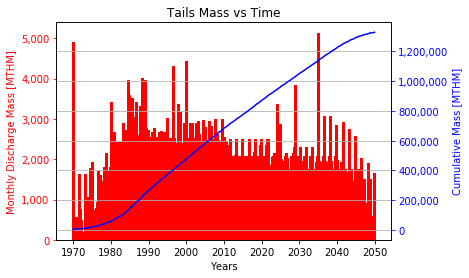
\includegraphics[scale=0.7]{./images/eu_future/tails.png}
    \end{center}
        \caption{Simulated accumulation of tails in the \gls{EU} is shown as a function of time.}
    \label{fig:eu_tail}
\end{figure}

\begin{figure}[htbp!]
    \begin{center}
        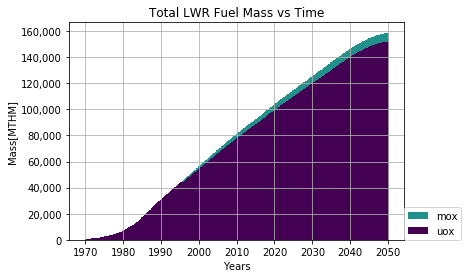
\includegraphics[scale=0.7]{./images/eu_future/total_fuel.png}
    \end{center}
\caption{Simulated total \gls{EU} fuel usage is shown as a function of time.}
    \label{fig:eu_fuel}
\end{figure}


\begin{figure}[htbp!]
    \begin{center}
            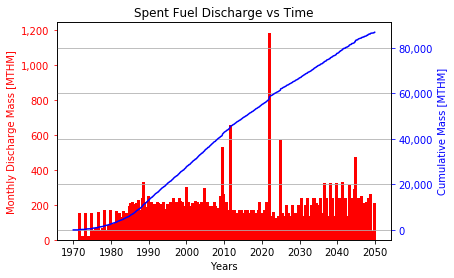
\includegraphics[scale=0.7]{./images/eu_future/snf_discharge.png}
    \end{center}
        \caption{Simulated \gls{EU} \gls{UNF} accumulation and discharge is 
shown as a function of time.}
    \label{fig:eu_snf}
\end{figure}

\FloatBarrier
\subsubsection{French \gls{SFR} Deployment}


Reprocessing the \gls{UNF} collected from all EU nations can provide the 
initial cores for approximately 180 \glspl{SFR}. Table \ref{tab:pu} lists the 
isotope, mass fraction, and quantity of plutonium that can be obtained from the 
2050 \gls{UNF} inventory.  With the \gls{SFR} breeding ratio above one, France 
can transition into a fully \gls{SFR} fleet without extra construction of 
\glspl{LWR}. 

\begin{table}[h]
    \centering
    \caption{Plutonium in the \gls{UNF} inventory.}
    \begin{tabular}{lrr}
        \hline
        \textbf{Isotope} & \textbf{Mass Fraction in Used Fuel [\%]} & \textbf{Quantity [t]} \\ \hline
        Pu238 & 0.0111 & 10.52 \\ 
        Pu239 & 0.518 & 545.05 \\ 
        Pu240 & 0.232 & 244.11 \\ 
        Pu241 & 0.126 & 132.58 \\ 
        Pu242 & 0.0487 & 51.24 \\ \hline
        \textbf{Total} & \textbf{0.9358} & \textbf{983.52} \\ \hline
    \end{tabular}
    
    \label{tab:pu}
\end{table}

From Varaine et al. \cite{varaine_pre-conceptual_2012}, a French
ASTRID-type 600\gls{MWe} \gls{SFR} consumes $1.225$ metric tons of
plutonium a year, with an initial plutonium loading of $4.9$ metric tons. 
Thus, the number of \glspl{SFR} that can be loaded with the reprocessed
plutonium from \gls{UNF} can be estimated to be 200, assuming adequate 
reprocessing and fabrication capacity as well as abundant depleted uranium 
supply.
 
Used \gls{MOX} from an ASTRID reactor is 23.95\% plutonium
in this simulation (see \cref{tab:comp}), whereas fresh \gls{MOX} is 22\% plutonium.
The plutonium breeding ratio in this simulation is thus assumed to be
$\approx 1.08$.

\Cref{fig:fuel} shows MTHM of \gls{MOX} loaded in the \glspl{SFR} per month.  The plot 
has peaks during a period of aggressive deployment of \glspl{SFR} followed by 
an equilibrium at 100 \gls{MTHM}. The peaks reoccur with the deployment of the 
second generation of \glspl{SFR}.  The spikes are due to initial fuel demand 
correspoding to these new deployments.  The initial cores loaded into new 
\glspl{SFR} rely on the \gls{MOX} created from legacy \gls{UNF}. Once the 
deployed \glspl{SFR} create enough extra plutonium, the legacy \gls{UNF} is no 
longer used. Notably, this switch from a less preferred fuel origin to a more 
preferred fuel origin is handled automatically within \Cyclus via user-defined preferences 
within its dynamic resource exchange algorithm \cite{gidden_methodology_2016}.


\begin{figure}[htbp!]
    \begin{center}
        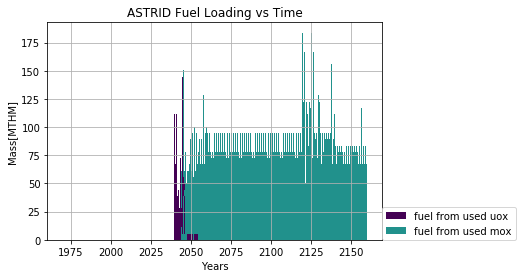
\includegraphics[scale=0.7]{./images/french-transition/where_fuel.png}
    \end{center}
    \caption{Fuel loaded into \glspl{SFR} was simulated in discrete 
        batches.}
    \label{fig:fuel}
\end{figure}

\Cref{fig:pu_no_cum} shows the separated plutonium discharge per month from the reprocessing plant. The plutonium outflux does not precisely follow the fuel demand because \Cyclus agents have material buffers that store commodity fuel for later usage. The reprocessed plutonium from legacy \gls{UNF} is stored for the initial loading of \glspl{SFR}.  Plutonium separated from legacy \gls{UNF} meets plutonium demans sufficiently to reduce the reprocessing demand for the first aggressive deployment of \glspl{SFR}.  The plutonium from reprocessing legacy fuel is a flat rectangle because the reprocessing throughput was set to 183.2 $\frac{\gls{MTHM}}{month}$ to avoid reprocessing all the legacy in one timestep. 
 

\begin{figure}[htbp!]
    \begin{center}
        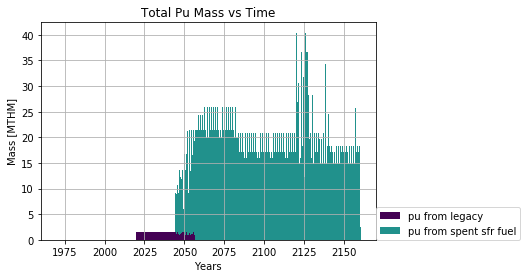
\includegraphics[scale=0.7]{./images/french-transition/pu.png}
    \end{center}
    \caption{The separated plutonium discharge from the reprocessing plant 
        in $\frac{\mbox{MTHM}}{\mbox{month}}$.}
    \label{fig:pu_no_cum}
\end{figure}

\Cref{tab:sfr_sim_result} lists metrics obtained from the second simulation.

\begin{table}[h]
    \centering
    \caption {In the French transition to \glspl{SFR},
                  the total legacy \gls{UNF} reprocessed is the 
                                  amount of \gls{UNF} France needs 
                  for a transition into a fully \gls{SFR} fleet. 
                                  %The tails used is around ninth of the original tails inventory from the previous simulation.
                                  %KDH note: What does this mean?
                                  %thought there was only one simulation. . . 
                          }
    \scalebox{1}{
        \begin{tabular}{llr}
            \hline
            \textbf{Category} & \textbf{Unit} & \textbf{Value}  \\ \hline
            Total \gls{ASTRID} MOX used & MTHM & 63,447  \\ 
            \textbf{Average UOX Reprocessing} & MTHM/month & \textbf{123.27} \\
            \textbf{Average Total Reprocessing} & MTHM/month & \textbf{63.23} \\
            \textbf{Average Fuel Fabrication} & MTHM/month & \textbf{74.31} \\
            Total \glspl{SFR} Deployed & & 220 \\ 
            Total Plutonium Reprocessed & MTHM & 14,831 \\ 
            Total \gls{ASTRID} fuel from UOX Waste & MTHM & 2,895  \\ 
            Total \gls{ASTRID} fuel from MOX Waste & MTHM  & 60,552 \\ 
            Total Tails used & MTHM & 49,488 \\ 
            \textbf{Total legacy UNF reprocessed} & MTHM & \textbf{53,595} \\ 
            Total Reprocessed Uranium Stockpile & MTHM & 159,383 \\ 
            Total Raffinate & MTHM & 24,789 \\ \hline
        \end{tabular}}
        
        \label{tab:sfr_sim_result}
\end {table}

\FloatBarrier

These results demonstrate that despite the large amount of initial plutonium that has to be reprocessed
prior to \gls{ASTRID} deployment, the 20 years (2020-2040) of 
\gls{ASTRID} fuel preparation
allows a reasonable level of average
\gls{UOX} reprocessing capacity demand. \gls{UOX} reprocessing continues 
until 2057, when the \gls{ASTRID} spent fuel can supply the plutonium
for its own fuel.

\section{Sensitivity Analysis}

I explored the impact of two key variables, the lifetime of French
\glspl{LWR} and the breeding ratio of \gls{ASTRID} reactors. The range
of these parameters (\cref{tab:sen_par}) sought to capture the full
span of their uncertainty.


\begin{table}[h]
    \centering
    \caption{Both \gls{LWR} lifetime and \gls{ASTRID} breeding ratio impact 
    transitional reprocessing demand.}
    \begin{tabularx}{0.8\textwidth}{lrr}
        \hline
        \textbf{Parameter} & \textbf{Default} & \textbf{Values} \\
        \hline
        Breeding Ratio of \glspl{ASTRID} & 1.08 & 1.11, 1.15, 1.18 \\ 
        Lifetime of French \glspl{LWR} [years] & 60  & 65, 70, 80 \\
        \hline
    \end{tabularx}
    \label{tab:sen_par}
\end{table}

\subsection{Breeding Ratio}

Increase in the breeding ratio of \gls{ASTRID} reactors
decreases the monthly \gls{LWR} \gls{UNF} reprocessing demand, as shown in 
figure \ref{fig:br_rep}. 
An increase in breeding ratio also reduces the number of total \gls{UOX} \gls{UNF}
required for the transition, because the \gls{ASTRID} creates more plutonium.
The demand previous to 2050 is unaffected by the 
breeding ratio because only \gls{UOX} \gls{UNF} is reprocessed. 

\begin{figure}[htbp!]
    \begin{center}
        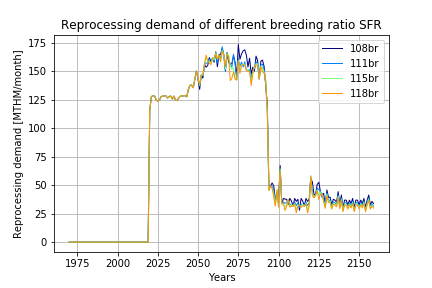
\includegraphics[scale=0.7]{./images/sensitivity/br_tot_rep.png}
    \end{center}
    \caption{Increasing the breeding ratio decreases the monthly reprocessing 
    demand.}
    \label{fig:br_rep}
\end{figure}


The sensitivity analysis also shows, as demonstrated in \cref{fig:br_uox} that 
increasing the breeding ratio decreases the mass of \gls{UOX} \gls{UNF} 
required for the transition. The \glspl{ASTRID} produce more plutonium, reducing the plutonium demand from reprocessed \gls{UOX}.

\begin{figure}[htbp!]
    \begin{center}
        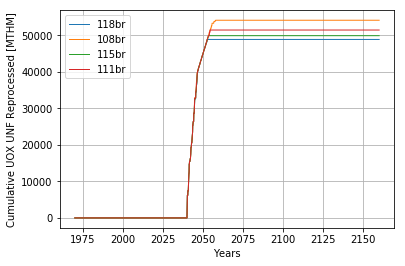
\includegraphics[scale=0.7]{./images/sensitivity/br_uox_unf_cum.png}
    \end{center}
    \caption{Sensitivity analysis demonstrates that increasing the breeding 
    ratio decreases the required \gls{UOX} \gls{UNF}. }
    \label{fig:br_uox}
\end{figure}

\FloatBarrier

\subsection{Lifetime Extension of French \glspl{LWR}}\label{sec:life}
Extending the lifetime of French \glspl{LWR} dramatically lowers the average
monthly \gls{UOX} reprocessing demand, since the \gls{ASTRID} deployment becomes 
delayed (shown in figure \ref{fig:pow_diff}). The plutonium demand is delayed,
 allowing the reprocessing plant more time to prepare plutonium for \gls{ASTRID} reactors.

\begin{figure}[htbp!]
    \begin{center}
        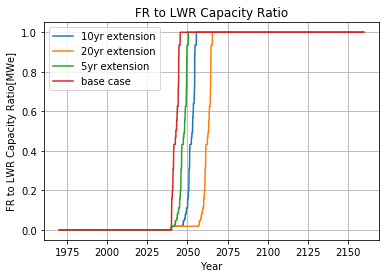
\includegraphics[scale=0.7]{./images/sensitivity/pow_ratio.png}
    \end{center}
    \caption{The ratio of \glspl{ASTRID} to \glspl{LWR} in France demarcates 
    the transition period.}
    \label{fig:pow_diff}
\end{figure}

 Increasing \gls{LWR} lifetimes also enables a less aggressive transition to 
 \glspl{ASTRID}. 
Figure \ref{fig:ext_uox} shows the decrease in the average monthly
\gls{UOX} reprocessing burden with increased \gls{LWR} lifetimes,
which reduces to the current capacity of the La Hague site if all the
French \glspl{LWR} extended their operation for 20 years.
However, figure \ref{fig:ext_all} shows that lifetime extension has little
effect on the average total monthly reprocessing demand, because
the amount of plutonium in the \gls{ASTRID} used fuel remains the same.
The initial increase is caused by the delay of \gls{ASTRID} deployment
delaying the first \gls{ASTRID} \gls{UNF} reprocessing. The period of which
\gls{ASTRID} \gls{UNF} is reprocessed decreases, which increases
the average.

\begin{figure}[htbp!]
    \begin{center}
        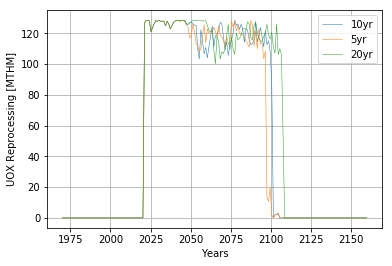
\includegraphics[scale=0.7]{./images/sensitivity/ext_uox_rep.png}
    \end{center}
    \caption{Increasing the lifetime of French \glspl{LWR} decreases the monthly
    \gls{UOX} reprocessing demand.}
    \label{fig:ext_uox}
\end{figure}


\begin{figure}[htbp!]
    \begin{center}
        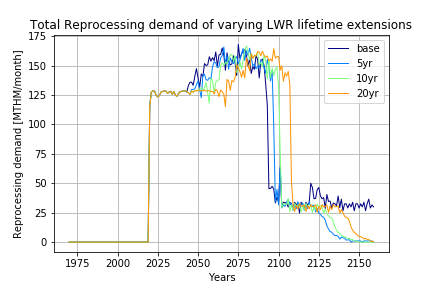
\includegraphics[scale=0.7]{./images/sensitivity/ext_tot_rep.png}
    \end{center}
    \caption{Increasing the lifetime of French \glspl{LWR} simply delays the
             reprocessing demand, and has little impact on the total 
     reprocessing capacity required.}
    \label{fig:ext_all}
\end{figure}
\FloatBarrier

\section{Conclusion}

France can transition into
a fully \gls{SFR} fleet with installed capacity of 66,000 \gls{MWe} without
building additional \glspl{LWR}
if France receives \gls{UNF} from other \gls{EU} nations.
Supporting the \gls{SFR} fleet requires an average 
reprocessing capacity of 73.27 \gls{MTHM} per month,
and an average fabrication capacity of 45.29 \gls{MTHM} per month.

Since most \gls{EU} nations do not have an operating \gls{UNF}
repository or a management plan, they have a strong incentive
to send their \gls{UNF} to France. In particular, the nations
planning aggressive nuclear reduction will be able phase out nuclear
without constructing a permanent repository. France has an
incentive to take this fuel, since recycling used fuel from
other nations will allow France to meet their MOX demand
without new construction of \glspl{LWR}.

\Cref{tab:which_send} lists \gls{EU} nations and their \gls{UNF} inventory
in 2050. We analyzed a strategy in which 
the nations reducing their nuclear fleet send their \gls{UNF} to France.
The sum of \gls{UNF} from Italy, Slovenia, Belgium, Spain and Germany
provides enough \gls{UNF} for the simulated transition ($\approx 54,000$ MTHM). 
These nations are shown in bold in \cref{tab:which_send}.
Sweden is not considered because of its concrete waste management plan.


\begin{table}[h]
    \centering
    \caption {\gls{EU} nations and their respective \gls{UNF} inventory.} 
                \begin{tabular}{llr}
                    \hline 
                    \textbf{Nation} & \textbf{Growth Trajectory} & \small{\textbf{UNF in 2050 [MTHM] }}\\
                    \hline
                    Poland & Aggressive Growth & 1,807\\
                    Hungary & Aggressive Growth & 3,119 \\ 
                    UK & Aggressive Growth & 13,268\\
                    Slovakia & Modest Growth & 2,746\\
                    Bulgaria & Modest Growth & 3,237 \\
                    Czech Rep. & Modest Growth & 4,413\\
                    Finland & Modest Growth &  5,713\\
                    Netherlands & Modest Reduction & 539\\
                    \textbf{Italy} & \textbf{Modest Reduction} & \textbf{583}\\
                    \textbf{Slovenia} & \textbf{Modest Reduction} & \textbf{765}\\
                    \textbf{Lithuania} & \textbf{Modest Reduction} & \textbf{2,644} \\
                    \textbf{Belgium} & \textbf{Aggressive Reduction} & \textbf{6,644}\\
                    \textbf{Spain} & \textbf{Modest Reduction} &  \textbf{9,771} \\
                    \textbf{France} & \textbf{Modest Reduction} & \textbf{9,979} \\
                    Sweden & Aggressive Reduction & 16,035\\
                    \textbf{Germany} & \textbf{Aggressive Reduction} & \textbf{23,868}\\
                    \hline
                \end{tabular}
    
    \label{tab:which_send}

\end{table}

On the other hand, in these simulations, some complex political and economic factors were not incorporated and various assumptions were present in this scenario. For
example, Germany's current policy is to not reprocess its \gls{LWR} fuel
\cite{topfer_germanys_2011}, and this policy would create a shortage
in the supply of \gls{LWR} \gls{UNF} for \gls{ASTRID} \gls{MOX} production.
Continuation of that German policy would not, however, be incompatible
with a change in \gls{EU} policy that frees \gls{EU} countries from
creating their high level waste repositories, since France could still
agree to take in Germany's \gls{UNF} for direct disposal. The analysis
method described herein could readily be adapted to account for such possibilities. 
The collaborative option explored here may hold value for the \gls{EU} nuclear community,
and may enable France to advance more rapidly into a closed fuel cycle. 
\FloatBarrier